\documentclass[11pt, conference]{IEEEtran}
\IEEEoverridecommandlockouts
% The preceding line is only needed to identify funding in the first footnote. If that is unneeded, please comment it out.
\usepackage{cite}
\usepackage{amsmath,amssymb,amsfonts}
\usepackage{algorithmic}
\usepackage{graphicx}
\usepackage{textcomp}
\usepackage{xcolor}
\usepackage{kotex}
\usepackage{booktabs}
\usepackage{tabularx}
\usepackage{supertabular,booktabs}
\usepackage{adjustbox}
\usepackage{enumitem}
\usepackage{romannum}
\usepackage{makecell}
\usepackage{multirow}
\usepackage{hyperref}
\usepackage{graphics}
\usepackage{subfigure}
\usepackage{float}
%\usepackage[outdir=./]{epstopdf}

\def\BibTeX{{\rm B\kern-.05em{\sc i\kern-.025em b}\kern-.08em T\kern-.1667em\lower.7ex\hbox{E}\kern-.125emX}}
\begin{document}

\title{IOT Home Heroes\\
\small{Seamless home automation based on posture/position detection\\}
}

\makeatletter
\newcommand{\linebreakand}{%
  \end{@IEEEauthorhalign}
  \hfill\mbox{}\par
  \mbox{}\hfill\begin{@IEEEauthorhalign}
}
\makeatother

\author{
  \IEEEauthorblockN{Jo Taesik}
  \IEEEauthorblockA{\textit{dept. of Information Systems} \\
    \textit{Hanyang University}\\
    Seoul, Korea\\
    r4pidstart@hanyang.ac.kr}
  \and
  \IEEEauthorblockN{Kwon Jongin}
  \IEEEauthorblockA{\textit{dept. of Information Systems} \\
    \textit{Hanyang University}\\
    Seoul, Korea \\
    whddlswhdaud@naver.com}
  \and
  \IEEEauthorblockN{Bae Hyojeong}
  \IEEEauthorblockA{\textit{dept. of Information Systems} \\
    \textit{Hanyang University}\\
    Seoul, Korea \\
    bhj09270@hanyang.ac.kr}
  \linebreakand % <------------- \and with a line-break
  \IEEEauthorblockN{Lee Hyunsuk}
  \IEEEauthorblockA{\textit{dept. of Information Systems} \\
    \textit{Hanyang University}\\
    Seoul, Korea \\
    leehyunsuk2000@gmail.com}
  \and
  \IEEEauthorblockN{Nan Haixu}
  \IEEEauthorblockA{\textit{dept. of Information Systems} \\
    \textit{Hanyang University}\\
    China, Guangzhou \\
    what-is-my-id@naver.com}
}

\maketitle
\begin{abstract}
\textit{With the recent surge in fascination with home automation, numerous companies are investigating strategies to facilitate the unified management of connected devices. A few of these techniques comprise verbal requests to a service for a particular action or the activation of a specific action when motion is sensed by designated sensors. Nevertheless, these approaches possess limitations that necessitate users to execute certain requests or actions that they would not typically perform to direct their devices. Devices also do not enable the full comprehension of the user's intentions. These restrictions do not meet the requirements of users who seek to construct home automation that can naturally recognize their intentions and respond correspondingly. Our proposal is to offer a service permitting users to initiate particular actions by way of genuine, intentional behavior that feels natural. This service offers a platform to assimilate and manage devices via the Matter protocol. On this platform, users can determine which actions are activated based on users interactions with certain objects in specific locations. By using IP cameras connected to the platform, OpenPose, Library for pose estimation assesses the user's posture, labelling it as sitting, lying down, standing, and more. By recognizing the posture of the user and specific objects, pre-defined actions are triggered. With this service, User can advance beyond traditional home automation to create a system that operates by comprehending user's intents with greater precision.\\}
% 최근 홈 오토메이션에 대한 관심이 높아짐에 따라, 여러 기업들은 연결된 기기를 통합적으로 간편하게 제어하기 위한 방법을 연구하고 있습니다. 음성으로 서비스를 호출하여 특정 액션을 요청한다던지, 특정 센서에 움직임이 감지되면 특정 액션이 트리거되는 등의 방법이 존재합니다. 그러나 이러한 방법들에는 한계가 존재합니다. 사용자로 하여금 기기를 제어하기 위해서가 아니라면 하지 않았을,  특정한 호출이나 동작을 강제합니다. 또한 사용자가 진정으로 무엇을 의도하는지 알 수 없다는 점도 있습니다. 이러한 한계는 자연스럽게 내 의도를 파악하여 그에 맞는 행동을 하는 홈 오토메이션을 구축하길 원하는 사용자들의 니즈를 충족시킬 수 없습니다. 그래서 우리는 사용자들이 부자연스럽지 않은, 의도가 담긴 자연스러운 동작을 통해 특정 액션을 트리거할 수 있는 서비스를 제안합니다. 이 서비스는 Matter 프로토콜을 이용해 기기들을 통합하고, 관리할 수 있는 플랫폼을 제공합니다. 이 플랫폼에서, 유저는 어느 위치의 어떤 사물에서 어떤 동작을 취하는지에 따라 어떤 액션이 트리거될 지를 설정할 수 있습니다. 이 플랫폼에 연결된 카메라를 이용해, openpose가 유저의 자세를 추정합니다. 이때 앉거나, 눕거나, 일어나는 등으로 유저의 자세를 분류합니다. 이런 방법으로 지정된 사물에서 설정해놓은 자세를 취하는 것을 인식하면 미리 지정된 액션을 트리거합니다. 이 서비스를 이용해 유저는 기존의 홈 오토메이션보다 한 단계 앞서 작동하고, 유저의 의도를 더욱 더 잘 파악하여 동작하는 홈 오토메이션을 완성할 수 있습니다.
\end{abstract}

\begin{IEEEkeywords}
home automation, IOT, Matter, pose estimation, OpenPose \\\\
\end{IEEEkeywords}

\large{Role Assignments}
\begin{table}[H]
\center
\begin{tabular}{m{1.4cm} m{1.5cm} m{4cm}}
\toprule
Roles & Name & Task description \& etc.\\
\midrule
User & Bae Hyojeong & He expects that he will be able to use them to make his life easier by operating IOT devices, However, He is hesitant because of the negative reviews from people who have already used them, or he is afraid that it will be too difficult to install and set them up. \\\\
Customer & Kwon Jongin & Created a product that can be controlled using IOT, but consumers rarely use the feature because it's not as convenient as expected. He is looking for ways to make his product more convenient to use in order to get consumers to use his product. \\\\
Software developer & Lee Hyunsuk, Nan Haixu & Designs and implements a solution to a given problem. Able to troubleshoot problems that may arise during development and complete assigned tasks within a given timeframe. \\\\
Development manager & Jo Taesik & Breaking down a given task into solvable problems and distributing them appropriately among team members. They also coordinate schedules to ensure that tasks are completed within a given timeframe. \\\\
\bottomrule
\end{tabular}
\end{table}
\newpage

\section{\Large{Introduction}}
% \begin{enumerate}[label=\arabic*]
%%%%%%%%%%%%%%%%%%%%%%%%%%%%%%%%%%%%%%%%%%%%
\subsection {\large{Motivation}} 
The IOT market has been growing rapidly in recent years. According to IOT Analytics, the IOT device market, which was valued at \$120 billion in 2019, is growing at a staggering rate, reaching \$100 billion in the first quarter of 2023. This market is also expected to grow at a CAGR of 20\% in the future. According to the same organization, there are currently an estimated 14.4 billion connected IOT devices, which is also expected to grow at a CAGR of 16\%. \\\\

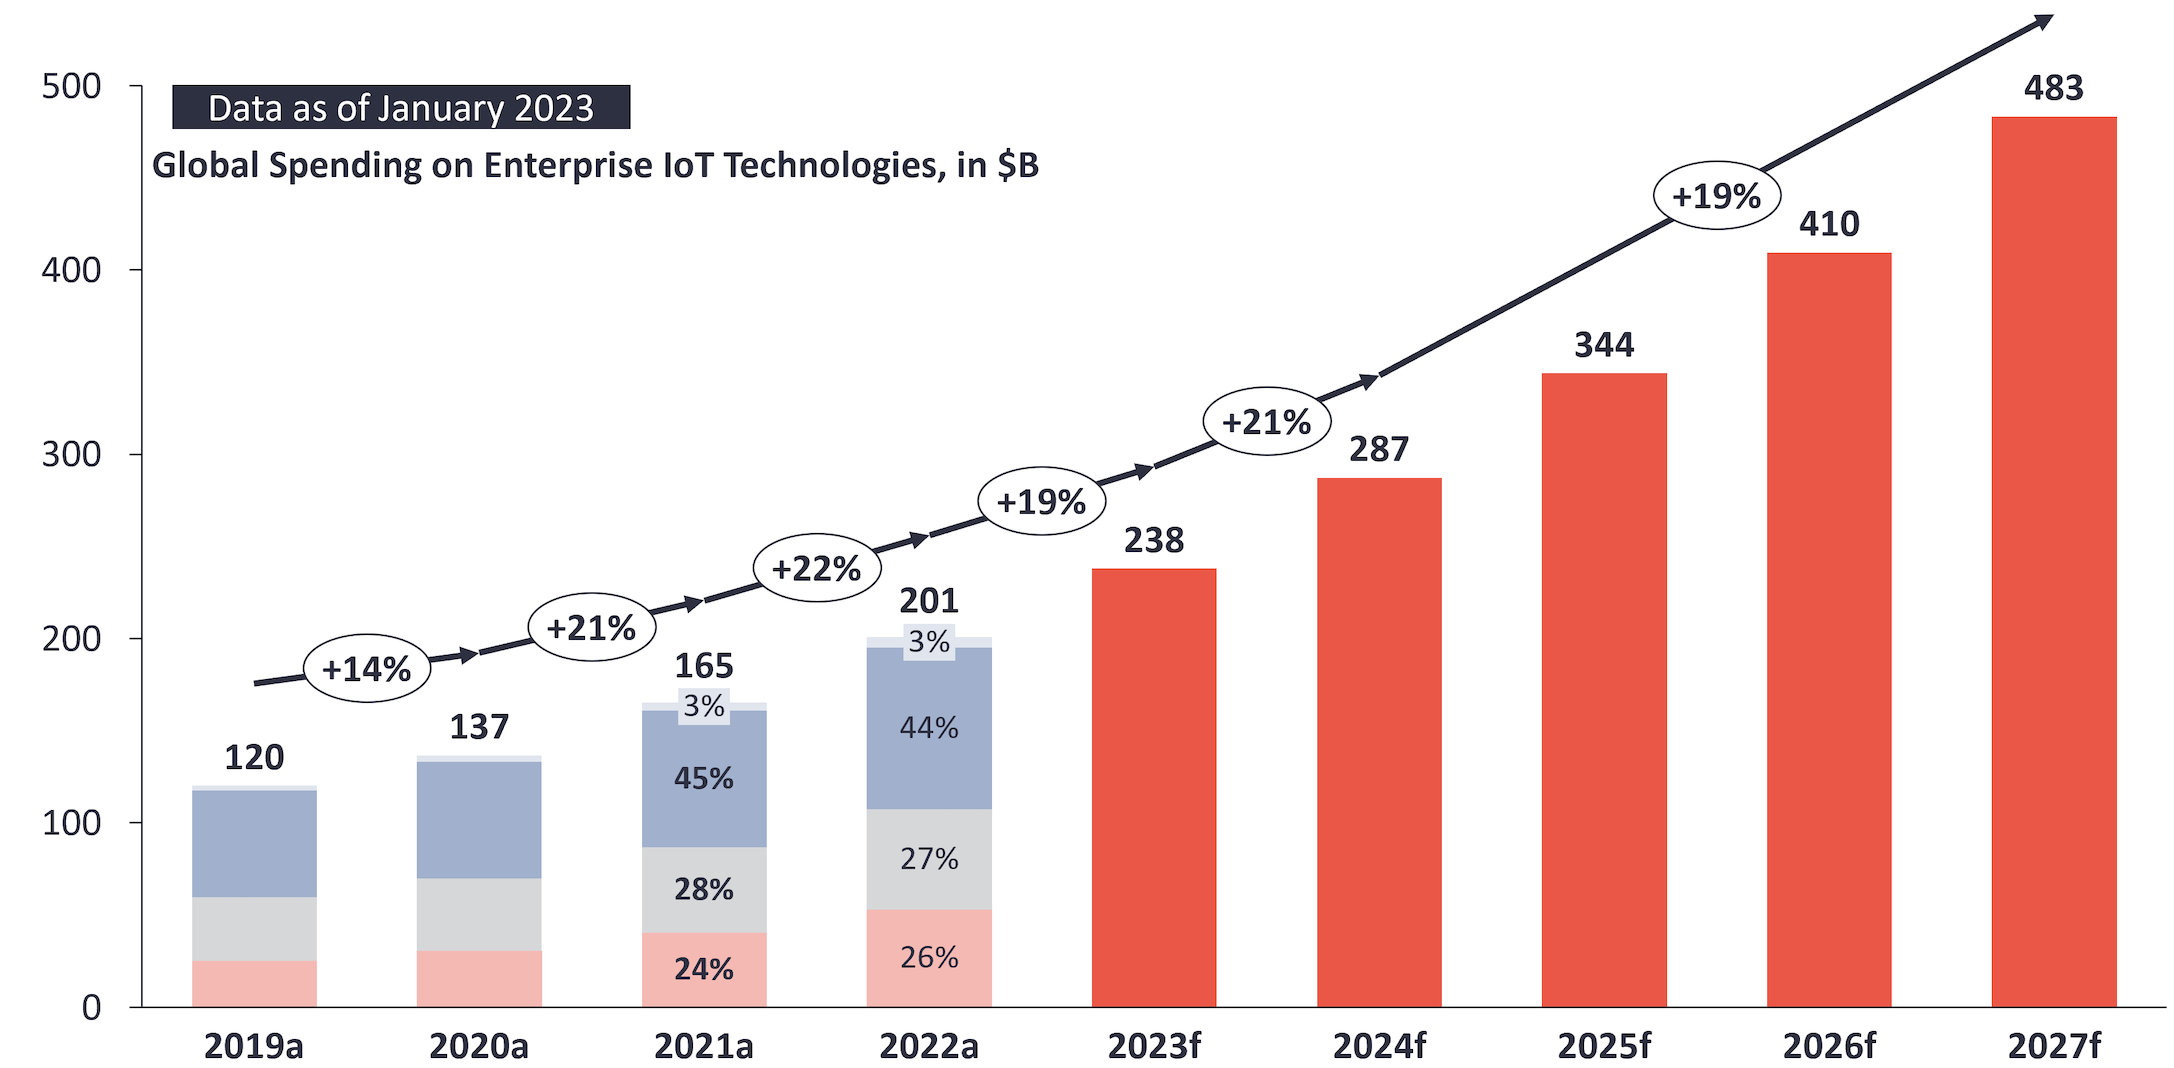
\includegraphics[width=8cm]{imgs/iot_market_growing.png}\\\\

In response to this market growth, many electronics manufacturers have begun to include IOT-related technologies in their products, ranging from passive technologies that allow you to control your device through an application on your phone, to technologies that allow you to control multiple devices with a single device in conjunction with devices such as smart speakers, to more advanced technologies such as air quality sensors and motion recognition sensors that allow you to operate your device automatically without human command. \\

Consumer interest in IOT technologies is on the rise, and according to OpenSurvey, the number of consumers who own a home appliance with these technologies has grown from 29.5\% in 2022 to 48.3\% in 2023, an increase of 18.8 percentage points over the previous year. \\\\

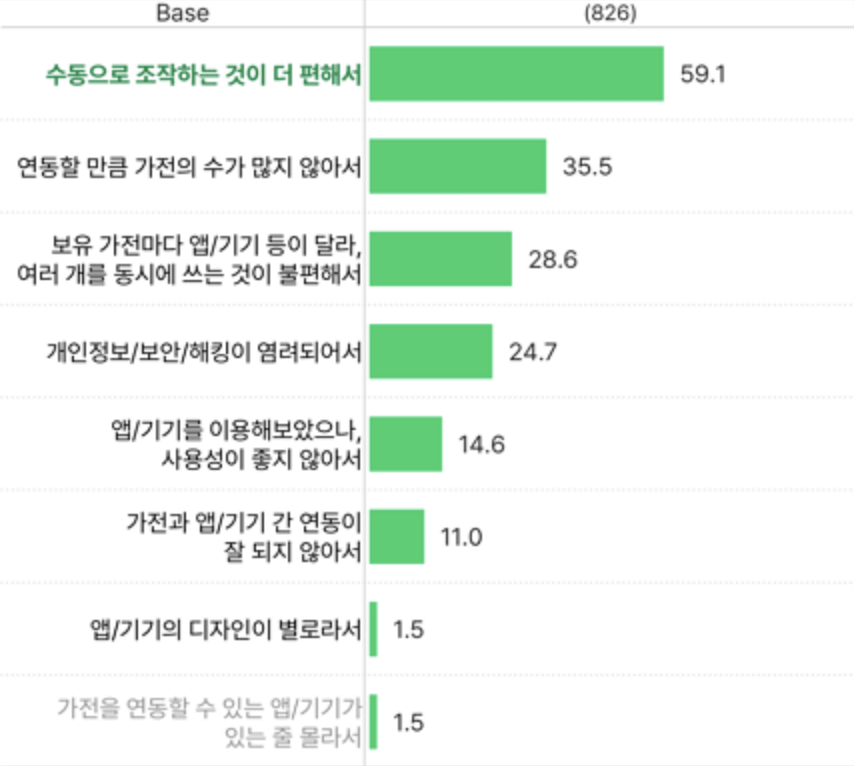
\includegraphics[width=8cm]{imgs/reason_why_not_use_iot.png}\\\\

However, consumers who have tried these technologies are often disappointed with devices that don't deliver on their pre-purchase expectations and stop using them. There are a few main reasons why this happens. According to OpenSurvey, these are the top reasons consumers have IOT devices but don't use them.\\
\begin{enumerate}
    \item They are more comfortable operating them manually (59.1\%)\\
    \item They have different apps/devices for each device they own and don't want to use multiple devices at the same time (28.6\%)\\
    \item They have tried the apps/devices but don't like the usability (14.6\%)\\
    \item The apps/devices don't work well with their devices (11.0\%)\\
\end{enumerate}

We propose a platform to address the necessary issues for consumers to utilize IoT technologies. Our integrated IoT platform employs posture recognition to activate desired functions.\\\\
%%%%%%%%%%%%%%%%%%%%%%%%%%%%%%%%%%%%%%%%%%%%
\subsection {\large{Problem Statement}}
    \begin{enumerate}[label=\alph*]
        \item Uncomfortable Automation\\
        There is a gap between what users think home automation should be and what current platforms offer. Users assume that machines will interpret their intentions and complete tasks without any input, but the reality is quite the opposite. The machines can only perform specific procedures that have already been entered, and they lack the ability to determine when those procedures should be executed. Currently, the sole means of inducing a machine to execute a task is through summoning a voice assistant with a designated command and directing it to execute a specific procedure. This hindrance fosters the belief that it is more convenient to manually operate a device than to avail oneself of automation. Consequently, users will avail themselves of IOT features only under highly restricted circumstances.\\
        
        \item Complexity of Use\\
        Currently, IOT devices from manufacturers and platforms can only be controlled through voice recognition. However, this method is too limited for users who desire a fully-fledged smart home. Third-party platforms exist for these users, which provide more detailed and advanced features. Although these platforms are not officially supported by the manufacturers, users who encounter problems must solve them on their own. Connecting devices to the platform and building the server are required tasks. Additionally, these platforms these platforms describe their behavior in code, which means users have to get used to it. These factors increase complexity and may present a barrier to entry for the users.\\
        
        \item Security Concerns\\
        Devices that use a manufacturer's platform can pose security risks by sending all user and device information to the manufacturer's servers. This compromise exposes sensitive personal information and lifestyle details to potential exploitation. Additionally, it opens up the possibility for malicious actors to manipulate and misuse devices in the home remotely.\\
        
        \item Disjointed communication methods\\
        Numerous communication methods are utilized in IoT devices these days, encompassing traditional WiFi and Bluetooth as well as UWB, RFID, Zigbee, Z-WAVE, XBee, LoRa, SigFox, and many others. Device manufacturers have selected one or more communication methods to construct their devices, resulting in consumers being limited to devices that use a specific communication method based on the hub they utilize.\\
        
        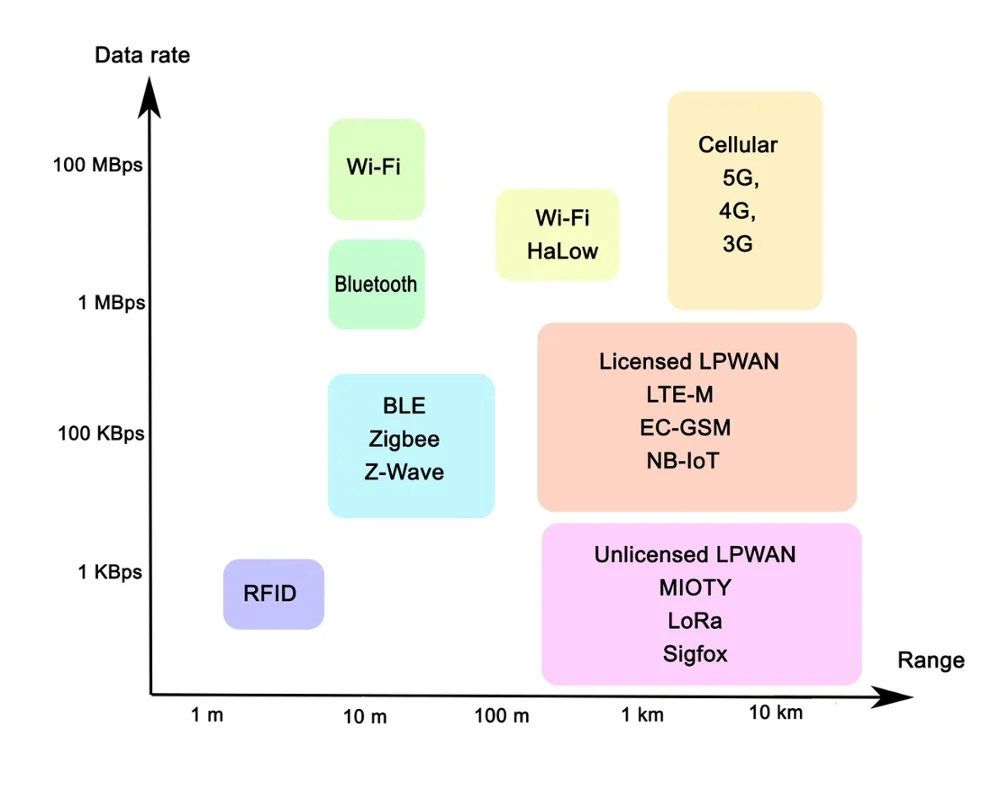
\includegraphics[width=8cm]{imgs/iot-protocols-1.png}\\\\
        
        \item Fragmented Platforms\\
        IOT device manufacturers maintain distinctive platforms and require navigating their platforms and hubs for using a specific device of a manufacturer. This limitation restricts the full functionality of devices to the manufacturer's designated platform, rendering interoperability difficult. Some manufacturer hubs do not allow devices from other manufacturers to connect, causing consumers to lean towards one manufacturer for their smart home devices and discouraging the use of products from different manufacturers at the same time. It also creates challenges when replacing a product line that is not made by a particular manufacturer, thus limiting consumer options.\\
        
    \end{enumerate}
%%%%%%%%%%%%%%%%%%%%%%%%%%%%%%%%%%%%%%%%%%%%
\subsection {\large{Related Software}}
    \begin{enumerate}[label=\alph*]
    \item Google Home\\
    This is a smart home platform offered by Google. It is compatible with a variety of devices, including lights, thermometers, speakers, and more. Additionally, it works with the Google Assistant, which allows you to check the status of your devices or control them. The same can be done through the accompanying application. Routines tailored to specific circumstances can be created and activated via voice commands. Easily add family members to share routines and jointly control devices. In addition to setting things up in the application, user can automate the details using YAML scripts.\\\\

    \item Apple Home\\
    This is a smart home platform offered by Apple that is compatible with a variety of devices including lights, thermometers, and speakers, among others. It works with the Siri, which allows you to check the status of your devices or control them. The same can be done through the accompanying application. One can conveniently monitor device status via Control Center or widgets on other Apple devices. An Apple TV can also serve as a hub and automatically regulate devices based on circumstance, including weather, motion, or humidity. However, an Apple device is required.\\\\

    \item Samsung Smartthings\\
    This is a smart home platform offered by Samsung. This platform is compatible with a variety of devices, including lights, thermometers, and speakers. Users can access and manage device status via Bixby or the application. To take full advantage of the IOT capabilities of their Samsung home appliances, users need this platform. User can utilize their Samsung devices as sensors. Unlike platforms offered by other manufacturers, Smartthings is an open platform, allowing for connection of even unsanctioned products through various actions. The hub permits connection of third-party sensors and setup of automation routines.\\\\

    \item LG ThinQ\\
    This is a smart home platform designed by LG that is necessary for full utilization of the IOT features of LG appliances. Users can receive notifications when their appliances finish their tasks, diagnose problems with their appliances, and schedule after-sales services. They can also integrate with Apple HomeKit to monitor or control their HomeKit-connected devices using this application.\\\\

    \item Home Assistant\\
    This is the sole mainstream smart home platform founded on open-source principles. The software can be installed and run on various hardware, including Raspberry Pi or Odroid. Devices with Home Assistant behave as hubs once the software is installed. It supports a diverse range of protocols and easily connects to devices unsupported by it through multiple actions. It is more difficult to configure than other platforms, but after mastering it, scripts can be utilized to access any data from linked devices and automate actions in numerous ways.\\

    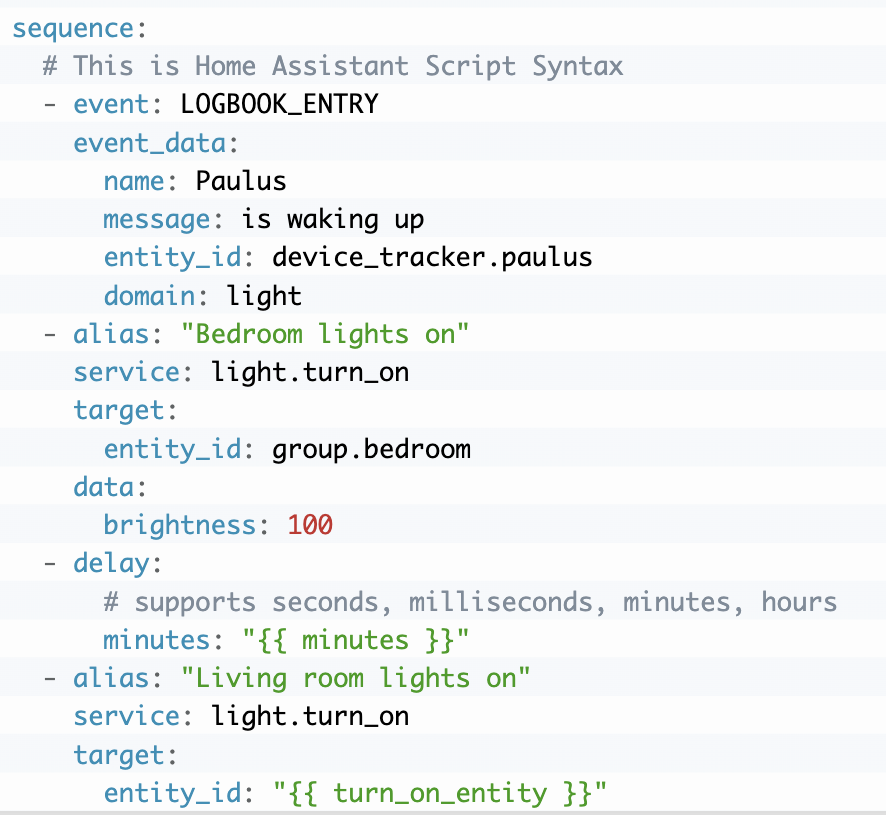
\includegraphics[width=8cm]{imgs/ha_script_example.png}\\\\
    \end{enumerate}

\section{\Large{Requirement Analysis}}
\begin{enumerate}[label=\arabic*]
    \item {\large{Login}}\\
    The user must log in to their own account, which contains their personal information. This application should be customizable for homeowners, so user’s personal information need to be stored in his/her own account. If the user manages multiple devices, the information is required for connecting to several devices. User can add and remove devices he/she manages. For the login process, user inputs their ID and password within the app, with the option to use the auto-login feature when needed. Alternatively, users can utilize an external ID, like a Google or Apple ID, to conveniently sign in without having to register.\\

    \item {\large{Logs and Statistics}}\\
    The application records user activities, including events such as login and logout, device control actions, and account management operations. It maintains device interaction logs, tracking device status changes, usage patterns, and scheduled events or automations triggered by the user. The application logs errors and exceptions, facilitating the identification of issues with error messages and timestamps. User behavior, preferences, and usage patterns are monitored to enhance this service. To achieve this, it stores a history of device status data, allowing users to review past device activities and monitor trends.\\

    \item {\large{Dashboard}}
    \begin{enumerate}[label=\alph*]
        \item {\large{Device connection}}\\
        The application stores and manages device connection information, including events such as device pairing and disconnection. It maintains logs of the connected devices, tracking the date and time of connection, the type of device, and the user responsible for the connection.\\
    
        \item {\large{Device Status Check}}\\
        The application logs device status, including the monitoring of device health, information about whether devices are connected or not and operational status. It maintains records of when status checks were performed, the specific devices checked, and the results, indicating whether devices were operational or reported issues.\\
    
        \item {\large{Device Control}}\\
        The application could control actions manually initiated by user. This events contain turning devices on or off, adjusting settings, and triggering automation sequences. It maintains logs of these control actions, capturing the user responsible, the devices affected, and the specific actions taken. Additionally, it tracks the timestamp of each control action for reference.\\



    \end{enumerate}

    \item {\large{Routine Managemant}}
    \begin{enumerate}[label=\alph*]
        \item {\large{Trigger Settings}}
            \begin{itemize}
              \item {\large{Sound Trigger}}\\
              Users can set conditions to trigger accessories or scenes based on sound intensity. For example, when a loud noise is detected at home, a message can be sent to the user. Or trigger a camera to capture what's going on. For speakers that can recognize voice, the response action can be completed according to the user's voice instructions.\\
              \item {\large{Sensor Trigger}}\\
              Response functions are triggered based on various sensors such as smoke alarms, flood alarms, motion sensor, air monitoring sensor. For example, if smoke is detected at home, a message can be sent to the user. Another example, The air purifier can be triggered automatically when the air quality declines.\\
              \item {\large{Time Trigger}}\\
              Accessories or scenes can be triggered based on a fixed time of day, certain days, or based on sunrise and sunset. For example, turn on the curtains and music at 6 a.m. every morning, or turn off all lights 15 minutes after sunset.\\
              \item {\large{Posture Recognition Trigger}}\\
              By obtaining images or videos through a camera and using OpenPose to recognize body posture, it is also possible to recognize body movements and trigger different functions based on different movements.\\
              \item {\large{Position Trigger}}\\
              The user's location can be determined based on the location information of the user's mobile phone, and corresponding functions can be triggered based on the user's location. For example, when the user returns home, they automatically turn on the lights and automatically start the air conditioner.\\
            \end{itemize}
    
        \item {\large{Behavior Settings}}\\

        
        b.1. The user must set the action to trigger through a specific trigger Action through gesture recognition in opencv above. \\
        
        For example, you have to be able to set the behavior of turning on the light, controlling the brightness, and how long the time interval is,\\

        b.2. More than one action light can be set with a single trigger, it must support collaboration between multiple devices, it must be user-generated,
        voice, sensor, time, and posture recognition should edit and delete the routine required for each trigger, and each user should be able to set the name of the routine and enable/disable the routine.\\
    \end{enumerate}

    \item {\large{Application Settings}}\\
    
    5-1. App Settings section, the user can set up the app. We need to implement this to initialize the setup data\\

    
    5-2. A push alarm on/off button must be implemented to determine whether or not to receive an alarm that alerts you when the routine is started by a particular trigger\\



    5-3. Each time each user logs in, backup and restore routes should be implemented without the need to create a new routine\\


5-4. The logout button should be implemented to enable account changes and a refresh function that allows users to set their own username
    
\end{enumerate}

\section{\Large{Development Environment}}
\begin{enumerate}[label=\arabic*]
    \item {\large{Task distribution}}
   
\end{enumerate}

\section{\Large{Specifications}}
\begin{enumerate}[label=\arabic*]
    \item {\large{Main}}
    \begin{enumerate}[label=\alph*]
        \item a
        \item b
        \begin{enumerate}
            \item aa
            \item ab
        \end{enumerate}
        \item c
    \end{enumerate}
    \item {\large{Main}}
    \begin{enumerate}[label=\alph*]
        \item a
        \item b
        \begin{enumerate}
            \item aa
            \item ab
        \end{enumerate}
        \item c
    \end{enumerate}
    \item {\large{Main}}
    \begin{enumerate}[label=\alph*]
        \item a
        \item b
        \begin{enumerate}
            \item aa
            \item ab
        \end{enumerate}
        \item c
    \end{enumerate}
    \item {\large{Main}}
    \begin{enumerate}[label=\alph*]
        \item a
        \item b
        \begin{enumerate}
            \item aa
            \item ab
        \end{enumerate}
        \item c
    \end{enumerate}
    \item {\large{Main}}
    \begin{enumerate}[label=\alph*]
        \item a
        \item b
        \begin{enumerate}
            \item aa
            \item ab
        \end{enumerate}
        \item c
    \end{enumerate}
    \item {\large{Main}}
    \begin{enumerate}[label=\alph*]
        \item a
        \item b
        \begin{enumerate}
            \item aa
            \item ab
        \end{enumerate}
        \item c
    \end{enumerate}
    \item {\large{Main}}
    \begin{enumerate}[label=\alph*]
        \item a
        \item b
        \begin{enumerate}
            \item aa
            \item ab
        \end{enumerate}
        \item c
    \end{enumerate}
    \item {\large{Main}}
    \begin{enumerate}[label=\alph*]
        \item a
        \item b
        \begin{enumerate}
            \item aa
            \item ab
        \end{enumerate}
        \item c
    \end{enumerate}
    \item {\large{Main}}
    \begin{enumerate}[label=\alph*]
        \item a
        \item b
        \begin{enumerate}
            \item aa
            \item ab
        \end{enumerate}
        \item c
    \end{enumerate}
    \item {\large{Main}}
    \begin{enumerate}[label=\alph*]
        \item a
        \item b
        \begin{enumerate}
            \item aa
            \item ab
        \end{enumerate}
        \item c
    \end{enumerate}
    \item {\large{Main}}
    \begin{enumerate}[label=\alph*]
        \item a
        \item b
        \begin{enumerate}
            \item aa
            \item ab
        \end{enumerate}
        \item c
    \end{enumerate}
    \item {\large{Main}}
    \begin{enumerate}[label=\alph*]
        \item a
        \item b
        \begin{enumerate}
            \item aa
            \item ab
        \end{enumerate}
        \item c
    \end{enumerate}
    \item {\large{Main}}
    \begin{enumerate}[label=\alph*]
        \item a
        \item b
        \begin{enumerate}
            \item aa
            \item ab
        \end{enumerate}
        \item c
    \end{enumerate}
\end{enumerate}


%     \item {\large{Choice of software development platform}}
%     \begin{enumerate}[label=\alph*]
%         \item development platform
%         \begin{enumerate}
%             \item Windows 10 : Windows are most commonly used operating system in Korea.  Among them, Windows 10, is used since Windows 11, the latest version, currently has stability problems.
%             \item Mac OS Monterey : It is a Unix-based operating system and it used to use the Xcode. Xcode verifies that the application is operating in an iOS environment. 
%             \item Android 6.0 \& up (api version 23 \& up) : Application test environment, developed with React Native, which is a cross platform. Minimum version follows Kakao Talk, which is supported in Android 6.0 \& up.
%             \item iOS 11 \& up : Among the application environments, iOS is used. Minimum version follows Kakao Talk, which is supported in iOS11 \& up.
%             \item Linux Ubuntu server 20.04 : Server environment which is driven by Amazon ec2 cloud computing service. Linux is optimized for running server in multi user operating system
%         \end{enumerate}
%         \item Language / Framework
%         \begin{enumerate}
%             \item Python / Django : \\
%             Python - multi-paradigm programming language that supports both procedure-oriented and object-oriented programming. Also, quick development can be made through simple grammar, dynamic typing and garbage collectors. \\
%             django - Through the vast amount of libraries that already exist, it is possible to develop repeated core functions quickly. In addition, user can solve problems quickly via official documents and other communities . It reduces the user's workload by creating database tables as classes.
%             \item Javascript / React Native v0.66 : \\
%             Javascript - Javascript is an interpreter or JIT compilation programming language that is widely used in script language for pages and non-browser environments such as Node.js. Users can obtain lots of reference materials in that javascript is the most commonly used programming language. \\
%             React Native : React Native is a cross-platform development tool that satisfies the conditions for supporting both Android and iOS operating systems since the expected application user is a household unit. With the concept of a component that emphasizes V among mvc patterns, fast development through code recycling is possible. Because it is client side rendering, front end developers can easily and actively develop. With large community, it is possible to solve problems quickly.
%             \item SQL : \\
%             SQL is created to manage data in a relational database system, which is used to directly access the database and modify data.
%         \end{enumerate}
%         \item Software 
%         \begin{enumerate}
%             \item Visual Studio Code : Widely used code editor, developed by Microsoft. It is a scalable code editor that provides convenient functions that exceed the level of code editors through a wide variety of extensions. We will be using extensions related to Django, Javascript and React.
%             \item Android Studio : Integrated development environment for Android development. We don’t use Android studios to write code, but we’re going to use Android simulators to be sure it works in Android. Or if it is necessary to utilize the Android native functions within React Native, we will use Android studio only in that part.
%             \item Xcode : Collection of OS X’s development tools developed by Apple. It will be used to test code written reactively in an iOS environment using an iOS simulator in it.
%             \item Git \& Github : Git is a distributed version management system that manages file change and tracking multi user's access, and Github is a web service that hosts these flag stores. Since we are developing both front and back ends by two team members, collaboration is important. So to prevent code collisions, we must check each other’s code. We will periodically integrate and manage code at remote storage through Github. Also, we will use git flow strategy to securely protect the integrated development  code while sustaining concurrency
%             \item Github Action : Github Action is a tool that automates CI/CD. Currently, we do not need to deploy continuously and thus we will mainly use CI automation. When a commit is detected, the committed code is inspected through a preset process to help continuous code integration management. Also various test sets already existing in Github Action enable CI automation.
%             \item Swagger :  Swagger is an open source software framework supported by a large tool ecosystem that helps developers design, build, document and consume REST web service. Since REST api does not have standardized conventions, front end developers should always check the specifications of api according to back-end developers. We will define api standards more easily and check api standards through swagger. 
%             \item Notion : Multipurpose recording tools can create their own systems for knowledgement management, memo writing, data management and project management. We will manage the schedule using our own project schedule management template in Notion. We plan to adopt the agile method and build new sprints every 3 days for speedy development.  
%             \item MySQL8.0.27 : Relational database system which has a framework for storing data. Since our application stores a large amount of user carbon emissions in format, MySQL has advantages. Also, MySQL is a frequently used program among RDBMS and since we learned this in our major, we can implement it quickly.
%             \item MySQL workbench : Program that can manage database creation in MySQL and single development integration environment via GUI. It can develop databases easily through graphic based interaction and database schema through reverse engineering.
%             \item Tensorflow \: Tensorflow is an open-source machine learning system developed by Google in 2015. Python allows you to develop artificial intelligence easily and quickly, and you can easily develop top artificial intelligence models through a large amount of libraries that already exist. It is also suitable for our team, which needs to be developed quickly as a platform that is very good for abstraction and visualization. 
%             \item NUGU playbuilder : NUGU playbuilder is a tool that helps developing service that executes in NUGU speaker. It enables machine learning by setting indent and entity inside conversation, actions on conversation and expected conversation during the development. Since every procedure of service is in GUI, developers who are not used to AI development can easily work on the service.\\
%             \end{enumerate}
%     \end{enumerate}
    
%     \item {\large{Software in Use}}\\
%     capture\\
%     Capture predicts monthly carbon emission based on car usage and diets and suggests 7\% of deduction. It has similarity with our service in that it predicts the emission and suggests goal deduction. But our service not only proposes goal reduction but also recommends practical actions and provides contents that help put it into action. Also our service communicates with AI speakers in the process, which brings out the action more effectively. \\
    
%     \item {\large{Cost}}
%     \begin{enumerate}[label=\alph*]
%         \item aws ec2  t2.micro : 0.0116 * 720(hour) = 8.352 dollars per month
%         \item Acrylic Plate 30,000 KRW
%         \item Half Mirror 25 Film 21,000 KRW
%         \item Roller 1,000 KRW
%         \item Sprayer 1,000 KRW
%         \item Display (20in.) 30,000 KRW
%         \item HDMI Cable 5,000 KRW
%         \item LAN Card 10,000 KRW
%         \item DVI to HDMI Converter 5,000 KRW
%         \item Micro SD Card 5,000 KRW
%         \item RASPBERRY-PI 3 B+ 70,000 KRW\\
%     \end{enumerate}
    
%     \item {\large{Task distribution}}
%     \begin{table}[H]
%     \centering
%     \begin{tabular}{m{3cm}|m{4cm}}
%     \toprule
%     Ko Byung Chan & Front end and back end \\
%     Yoona Chang Il & Front end and smart mirror\\
%     Jang Hyeong Jun & Back end and smart mirror\\
%     Choi Ha Young & AI and documentation\\
%     \bottomrule
%     \end{tabular}
%     \end{table}
% \end{enumerate}

% \section{\Large{Architecture Design \& Implementation}}
% \begin{enumerate}[label=\arabic*]
%     \item {\large{Overall Architecture}}\\
%     \begin{figure}[H]
%         \centering
%         \includegraphics[scale=0.2]{images/overallarchitecture.eps}
%     \end{figure}
%     This is the Our service consists of five modules. Each is front-end, back-end, database, machine learning, and IoT such as AI speaker and smart mirror. Among them, front-end and IoT are modules that directly communicate with users. \\
%     The first module is the front-end. We used JavaScript language and React Native, a cross-platform framework that supports both Android and IOS as a mobile application framework. So, all household members can use our application regardless of their smart phone model. Through the application, the user can belong to the household and check the appropriate carbon emission reduction behavior. In addition, users can check the amount of carbon they can reduce when they practice carbon emission reducing efforts in each behavioral area and the amount of carbon emission they are currently emitting in each behavioral area.\\
%     The second is the back-end. We used the Django framework based on the Python language as the web application server framework. In addition, uWSGI was used as wsgi middleware that connects web server and web application server. And nginx was used as the web server. The backend largely communicates with three devices: application, AI speaker, IoT such as smart mirror. So, the server is implemented in the form of providing REST API. When the AI speaker notifies the server that the user has started/ended the carbon emission reduction behavior, the server stores it to the database. Also, the server responds when the application requests the user’s information.\\
%     Third, it is a database.  We used mysql as a database. Mysql is an RDBMS, we store user information, user behavior practice records, information related to user behavior practice, and previous dataset statistics.\\
%     The fourth is machine learning. We predict the most appropriate shower shortcut time through the user’s first shower time. Reducing the shower time by 1 minute has a problem of presenting an absolute value without considering the shower time of the user. Therefore, there is a problem in that users try to reduce 1minute even though they can reduce more time without experiencing inconvenience. Therefore, we present an AI model that presents an appropriate reduction for the user’s shower time.\\
%     Lastly, it is IoT. We used AI speakers to interact with users by voice when practicing carbon emission reduction behavior, making it easier to use the service in more diverse situations. Voice interaction services are developed using existing development tools. In the case of smart mirrors, raspberry pie was used.\\
    
%     \item {\large{Directory Organization}}\\
%     \begin{enumerate}[label=\alph*]
%         \item front end
% \begin{flushleft}
%         \tablefirsthead{\toprule Directory & File name & etc \\}
%         \tablehead{\toprule Directory & File name & etc\\}
%         \tabletail{\midrule}
%         \tablelasttail{\bottomrule}
%         \begin{supertabular}{p{0.5\linewidth} | p{0.3\linewidth} p{0.05\linewidth}}
%         \midrule
%         /front-end & \makecell[l]{.eslintrc.js\\.gitignore\\.prettierrc.js\\.watchmanconfig\\app.json\\babel.config.js\\index.jsx\\package.json} \\
%         \midrule
        
%         /front-end/apps	& App.jsx \\
%         \midrule
        
%         /front-end/apps/assets & \makecell[l]{environmenttw.png\\globe.png\\globew.png\\logo.png\\logo2.png}\\
%         \midrule
        
%         \makecell[l]{//front-end/apps\\/navigator} & \makecell[l]{mainNavigator.jsx\\signInNavigator.jsx\\bottomTabNavigator.jsx}\\
%         \midrule
        
%         \makecell[l]{/front-end/apps\\/components/api} & axios.jsx\\
%         \midrule

%         \makecell[l]{/front-end/apps\\/components/common} & wrapper.jsx\\
%         \midrule
        
%         \makecell[l]{/front-end/apps\\/components/context} & tokenContext.jsx\\
%         \midrule
        
%         \makecell[l]{/front-end/apps\\/components/navigator} & \makecell[l]{bottomTabNavigator.jsx\\ GraphDetailsNavigator.jsx\\graphNavigator.jsx\\loginNavigator.jsx\\mainNavigator.jsx}\\
%         \midrule

%         \makecell[l]{/front-end/apps\\/components/screens\\/main} & main.jsx\\
%         \midrule
        
%         \makecell[l]{/front-end/apps\\/components/screens\\/signUp} & signUp.jsx\\
%         \midrule
        
%         \makecell[l]{/front-end/apps\\/components/screens\\/signIn} & signIn.jsx\\
%         \midrule
        
%         \makecell[l]{/front-end/apps\\/components/screens\\/home} & home.jsx\\
%         \midrule
        
%         \makecell[l]{/front-end/apps\\/components/screens\\/recommended} & recommended.jsx\\
%         \midrule
        
%         \makecell[l]{/front-end/apps\\/components/screens\\/records} & records.jsx\\
%         \midrule
        
%         \makecell[l]{/front-end/apps\\/components/screens\\/profile} & \makecell[l]{profile.jsx\\ myPageList.jsx}\\
%         \end{supertabular}
% \end{flushleft}
        
%         \item back end
%         \begin{flushleft}
%         \tablefirsthead{\toprule Directory & File name & etc \\ \midrule}
%         \tablehead{\toprule Directory & File name & etc\\ \midrule}
%         \tabletail{\midrule }
%         \tablelasttail{\bottomrule}
%         \begin{supertabular}{p{0.5\linewidth} | p{0.3\linewidth} p{0.05\linewidth}}
%         /server & \makecell[l]{.gitignore\\ manage.py}\\
%         \midrule
%         /server/app & \makecell[l]{\_\_init\_\_.py\\admin.py\\apps.py\\models.py\\serializer.py\\tests.py\\views.py}\\
%         \midrule
%         /server/config & \makecell[l]{\_\_init\_\_.py\\asgi.py\\settings.py\\urls.py\\wsgi.py}\\
%         \midrule
%         /server/app/migration & \makecell[l]{0001\_initial.py\\002\_auto\_2021\\        1126\_1010.py\\ \_\_init\_\_.py}\\
%         \midrule
%         /server/auth/migration & \makecell[l]{0001\_initial.py\\ \_\_init\_\_.py}\\
%         \end{supertabular}
% \end{flushleft}
        
%     \end{enumerate}
    
%     \item {\large{Module 1 : front end}}
%     \begin{enumerate}[label=\alph*]
%         \item Purpose\\
%         It is used to provide users with records of behavioral practices. It is also used to guide how to practice behavior. And it is to receive user information and manage household members.
%         \item Functionality\\
%         First of all, it provides a function of managing user information and household members, checking emissions for each behavior of the current user, and checking the amount of carbon that can be reduced. It also provides a function of checking average emissions in the group under the same conditions and checking carbon emission records due to daily and monthly behavior practice. Finally, it provides the function of checking how to practice carbon emission reduction behavior.
%         \item Location of Source Code\\
%         /front-end
%         \item Class Component
%         \begin{enumerate}
%             \item Main Page\\
%             It is the first component to be output when running the app. It is implemented as a functional component, and there is a style sheet representing css. The buttons in the component are imported from the common folder. The logo is imported from the assets folder.
%             \item Sign In Page\\
%             There is an inputText that receives an ID and password. The ID and password are managed through global variables within the file. When clicking the login button, put the ID and password in the request body and send a post request to the server.At this time, communication with the server uses the axios library and is processed asynchronously. React hooks are used to process asynchronous actions in functional components.
%             \item Sign Up Page\\
%             Because we need to receive a lot of information from the user over multiple pages when signing up, we manage multiple components within one file. This makes it easy to manage variables that have received user information without using additional status management libraries.
%             \item Home Page\\
%             This is the default routing page of the bottom tab bar. Page navigation was implemented through the React Navigation Library. The circular graph on the main page also used the graph library. The amount of emissions output in the screen is received through communication with the server when the page is first rendered.
%             \item Records Page\\
%             This page shows the daily and monthly records. Every time you click on that button, data is retrieved through communication with the server.
%             \item Recommended Action Page\\
%             When the user clicks on the list showing each behavior, it shows detailed information through modal. If you press the OK button, the modal window turns off. In the details, my emissions for the behavior, the average emissions of people in the same group as me, and the amount of carbon that can be reduced are output.
%             \item My Page\\
%             You can manage your information and household members on my page. At this time, only the householder is authorized to manage the household members. Permission status is processed by the server. The list of household members is implemented through the React flat list. In addition, the information received when modifying the information is managed as a global variable, and is delivered to the server when the modification button is clicked.
%         \end{enumerate}
%         \item Where it's taken from\\
%         Data is directly input by the user, or previous data is retrieved from db.
%         \item How/Why we used the module\\
%         React Native was used because it is a cross-platform framework that supports both Android and IOS. Since it mainly shows the user's record, it is used in the form of outputting the data when the user's data is retrieved from the server.
%     \end{enumerate}
    
%     \item {\large{Module 2 : back end}}
%     \begin{enumerate}[label=\alph*]
%         \item Purpose\\
%         Our service helps with various behaviors at home. Therefore, it should be linked with not only applications but also smart mirrors and AI speakers. For this reason, a server that manages many devices in an integrated manner was needed.
%         \item Functionality\\
%         It mainly provides REST APIs that respond to requests when sent from clients. When the client requests db's data, it inquires db and delivers the information to the client. Or it is in charge of communication between connected devices.
%         \item Location of Source Code\\
%         / server
%         \item Class Component
%         \begin{enumerate}
%             \item app/views.py\\
%             It is a part that is responsible for the core functions of our service, such as responding to user information requests and recording behavioral practices. This part is responsible for core business logic, and the view corresponding to the controller among the MVC patterns is implemented as a class-based view (CBV). Each function has each endpoint.
%             \item app/models.py\\
%             It is a file responsible for automatically connecting data from objects and databases. This makes it easier to access values in the database from Django. In this file, all tables in the database appear as objects.
%             \item app/serializer.py\\
%             This file serves to make the response value in the appropriate form to communicate with. All of the values modified in view are not in a bonded form to communicate with the client. Therefore, we need to make the value in an appropriate form. The client and server communicate in the form of JSON, so the serializer classes change the value to JSON form in this file.
%             \item config/urls.py\\
%             It is a file that manages endpoints for communication. It also connects endpoints and views. Endpoints for all requests are set here.
%         \end{enumerate}
%         \item Where it's taken from\\
%         In terms of data, data comes from applications, databases and various IoT such as AI speakers and smart mirrors.
%         \item How/Why we used the module\\
%         Django was used because it is a web application framework based on Python, the most common language. In addition, nginx and uWSGI were used to provide more stable services. The WAS was built in Django, and the web server was built in nginx. And they were connected by uWSGI.
%     \end{enumerate}
    
%     \item {\large{Module 3 : database}}
%     \begin{enumerate}[label=\alph*]
%         \item Purpose\\
%         We constructed a database to systematically store a lot of data generated when users practice carbon emission reduction behavior.  This is also because data with a fixed format must be stored steadily. So we chose MySQL, which is RDBMS. It is also for better AI modeling through data accumulation.
%         \item Functionality\\
%         It provides systematic data management through tables. In addition, relationships can be expressed through foreign keys between tables, enabling more efficient space management. In addition, we can easily manipulate a lot of data through query statements.
%         \item Location of Source Code
%         \begin{enumerate}
%             \item /server/app/models.py - we can check the DB in the form of ORM in the server directory. 
%             \item on aws rds
%         \end{enumerate}
%         \item Class Component
%         \begin{enumerate}
%             \item auth\_user\\
%             A table that stores user information. It is a user table provided by Django and can be easily expanded.
%             \item personalShowerData\\
%             A table that stores unchanged values among the user's shower data. It reduces the occurrence of duplicate values by distinguishing them from the shower log table.
%             \item showerLog\\
%             This is a table that stores the user's shower records. It regularly stores data every time a user takes a shower.
%             \item showerDataSet\\
%             This is the data based on the age group of the dataset. This is a table that we refer to when we need information about the same age as the user.
%         \end{enumerate}
%         \item Where it's taken from\\
%         It stores data input from the user. Or save behavioral records when the user practices behavior.
%         \item How/Why we used the module\\
%         First, we used user tables provided by 'Django'. Therefore, there were tables related to user information, and we expanded tables containing user behavior practice information from those tables. a table was created to store the user's behavioral practice records and a table to store invariant values such as the user's target shower time. And a table was created to store statistical content for datasets for ai learning.
%         \begin{figure}[H]
%             \centering
%             \includegraphics[scale=0.14]{images/database.eps}
%         \end{figure}
%     \end{enumerate}
    
%     \item {\large{Module 4 : machine learning}}\\
%     \begin{enumerate}[label=\alph*]
%         \item Purpose\\
%         Our service provides users the group’s carbon emission and the user’s predicted carbon reduction through the application. It invokes users to do the recommended action and set the target for them. Also users can comprehend the validity of the action and the number. In the process, machine learning is essential. \\
%         \item Functionality\\
%         Machine learning enables predicting new user’s carbon emission reduction. As the new application user downloads and signs in, data such as age and gender is sent to the database and his/hers reduction is predicted through the machine learning model we prepared.\\
%         \item Location of Source Code\\
%         ESG\_Home.ipynb
%         \item Class Component\\
%         \begin{enumerate}
%             \item train\_test\_split\\
%             It splits arrays or matrices into random train and test subsets, considering the parameters such as test\_size, train\_size and stratify.
%             \item StandardScaler\\
%             It standardizes features by removing the mean and scaling to unit variance. Standardization of a dataset is a common requirement for many machine learning estimators.
%             \item sklearn.metrics\\
%             It implements functions assessing prediction error for specific purposes. We used r2\_score, mean\_absolute\_error and mean\_squared\_error to evaluate and compare the models.
%             \item LinearRegression\\
%             Linear regression makes predictions by creating a linear function of training data.
%             \[ŷ = w[0] × x[0] + w[1] × x[1] + … + w[p] × x[p] + b\]
%             x[0] to x[p] is the feature and weight w and y-intercept b are parameters learned by the model
%             \item SGDRegressor\\
%             \begin{figure}[H]
%                 \centering
%                 \includegraphics[scale=0.1]{images/AI/sgd_pic.eps}
%             \end{figure}
%              Stochastic Gradient Descent (SGD) is a stochastic gradient descent method that randomly selects a sample from each step and calculates the gradient of the sample.\\
%              It has the advantage of being able to be applied to the large training dataset because it is repeatedly processed with small data and requires only memory for one sample.
%             \item LogisticRegression\\
%             Logistic regression is a supervised learning algorithm that predicts a probability that data falls into a category from 0 to 1 and predicts a category according to that probability. \\
%             Odds is the probability divided by the probability that an event has not occurred. In logistic regression, several features are multiplied by coefficients and intercepts are added to obtain and analyze the final value log-odds.\\
%             The logistic function, also called the sigmoid function, is a function that receives the log-odds obtained above as an input value and outputs a result value between 0 and 1. \\
%             We consider loss to ensure that logistic regression predicts the probability properly, i.e., whether the coefficients and intercepts obtained are appropriate. \\
%             Logistic regression can be seen as having high accuracy when this log loss value is minimized.
%             \item RandomForestRegressor\\
%             \begin{figure}[H]
%                 \includegraphics[scale=0.2]{images/AI/randforest_pic.eps}
%             \end{figure}
%             Random forest is a model that collects regression results from multiple decision trees configured through training and concludes.\\
%             Ensemble learning is a method of using multiple learning algorithms for overfitting prevention and high performance. Random forests initially generate trees through bagging. Bagging is the process of creating a decision tree by selecting some rows of training data, allowing overlapping of rows. Diversity is given to the decision tree by limiting the number of features to be used during this process, usually by the square root of the total number of attributes.
%             \item ExtraTreeRegressor\\
%             Extra trees, also called Extremely randomized trees, are even more random than random forests. Random selection of the number of data samples and feature selection increases prediction accuracy and prevents overfitting.
%             \item GradientBoostingRegressor\\
%             \begin{figure}[H]
%                 \centering
%                 \includegraphics[scale=0.3]{images/AI/gbr_pic.eps}
%             \end{figure}
%             Random forest is a model that collects regression results from multiple decision trees configured through training and concludes.\\
%             The main parameter of gradient boosting is the learning rate, a hyper-parameter that determines how strongly the error in the previous tree will be corrected. Increasing the learning rate creates a complex model because it strengthens correction. Also increasing the n\_estimator value adds more trees to the ensemble, complicating the model and fitting the train data more accurately. To prevent overfitting, you can reduce the depth of the tree or reduce the learning rate.
%             \item AdaBoostRegressor\\
%             AdaBoost is a model that adds weight to the results of other learning algorithms (weak learners). It is also used in combination with many other learning algorithms.\\
%             It is adaptive in that the weak learner can correct the results of incorrect analysis in the previous model. This makes them vulnerable to noise and outliers, but less vulnerable to overfitting than other learning algorithms.
%             \item XGBRegressor\\
%             \begin{figure}[H]
%                 \centering
%                 \includegraphics[scale=0.1]{images/AI/xgb_pic.eps}
%             \end{figure}
%             The Extreme Gradient Boosting model is a model that learns gradient boosting models in parallel.\\
%             Standard gradient boosting models do not have overfitting regulatory features, but XGBoost models are robust with its own overfitting regulatory features.
%             \item LGBMRegressor\\
%             Light GBM is a gradient boosting framework and is a tree-based learning algorithm. Unlike models that scale trees horizontally, LBGM grows trees vertically.\\
%             Even when dealing with large-sized data, memory usage is low, results are fast, and the results are focused on accuracy. LGBM is vulnerable to overfitting and is not used well in small datasets. Our data is a large dataset with 49.027 rows and thus we chose this model. The analysis showed a very high accuracy score, 99.99990470818714\%.
%             \item HistGradientBoostingRegressor\\
%             A histogram-based gradient boosting tree model, suitable for large datasets with more than 10,000 rows. It handles missing values on its own and determines whether the missing values should go to the left or right child during the training process. If missing values that were not in the training process appear during prediction, they are mapped to the child with the most samples.
%             \item permutation\_importance\\
%             It is a model inspection technique that can be used for any fitted estimator when the data is tabular. It is defined to be the decrease in a model score when a single feature is randomly shuffled. By breaking down the relationship between the feature and the target, the model score is indicative of how much the model depends on the feature.\\
%         \end{enumerate}
%         \item Where it's taken from\\
%         Based on the data we provide, models learned to predict the target, which here is reduction. And as the new user signs in, it receives the user’s data from our database and analyzes the reduction of the user.\\
%         \item How/Why we used the module
%         \begin{enumerate}
%             \item pandas\\
%             It’s a software library written for the Python programming language for data manipulation and analysis. In particular, it offers data structures and operations for manipulating numerical tables and time series.
%             \item io\\
%             The io module provides Python’s main facilities for dealing with various types of I/O. It enables reading files and printing outputs.
%             \item numpy\\
%             It is a library for the Python programming language, enabling large, multidimensional arrays and matrices, along with a large collection of high-level mathematical functions to operate on these arrays.
%             \item seaborn\\
%             It is a Python data visualization library based on matplotlib. It provides a high-level interface for drawing attractive and informative statistical graphics.
%             \item matplotlib.pyplot\\
%             It is a collection of functions that make matplotlib work like MATLAB. Each pyplot function makes some changes to a figure, such as creating a figure, creating a plotting area in a figure, plotting some lines in a plotting area and decorating the plot with labels.\\
%         \end{enumerate}
%     \end{enumerate}
    
%     \item {\large{Module 5 : AI speaker \& smart mirror}}
%     \begin{enumerate}[label=\alph*]
%         \item Purpose\\
%         There are many situations in the home where interaction through graphics is difficult, such as bathrooms. We provide voice-based interaction through AI speakers to make the service easier to use in these various situations. In addition, smart mirrors can induce more intuitive behavior to users.\\
%         \item Functionality\\
%         It helps to practice the action of reducing carbon emissions. For example, when the user informs the AI speaker of the start of the shower when taking a shower, the user's proper shower time appears as a timer on the smart mirror.\\
%         \item Location of Source Code
%         \begin{enumerate}
%             \item /smartMirror
%             \item AI speaker play builder\\
%         \end{enumerate}
%         \item Class Component
%         \begin{enumerate}
%             \item ask.showerStart\\
%             It's a place where AI speakers recognize a user's saying, "I'm going to start taking a shower." It is a place where AI speakers learn to recognize "I," "Shower," and "Start" as different entities.
%             \item ask.showerEnd\\
%             It's a place where AI speakers recognize a user's saying, "I finished taking a shower." It is a place where AI speakers learn to recognize "I," "Shower," and "finish" as different entities.
%             \item answer.showerStart\\
%             It is a file paired with ask.showerStart. Ask.showerStart is about recognizing the start of the shower, while answer.showerStart is about what the AI speaker should do after starting the shower.
%             \item answer.showerEnd\\
%             It is a file paired with ask.showerEnd. Ask.showerEnd is about recognizing the end of the shower, while answer.showeEnd is about what the AI speaker should do after the shower.
%             \item answer.showerSuccess\\
%             After the shower is completed, a praise message is output when the user successfully finishes the shower in time.
%             \item answer.showerFailed\\
%             After the shower is completed, a praise message is output when the user fails to finish the shower in time.
%             \item smartMirror/main\\
%             It is a file that implements a smart mirror. It is implemented based on the web and serves as a real mirror through raspberry pie. Basically, the current time and weather are output, and a shower timer is output at the start of the shower.\\
%         \end{enumerate}
%         \item Where it's taken from\\
%         AI speakers receive data directly from users. In the case of smart mirrors, data is received through the server.\\
%         \item How/Why we used the module\\
%         We created a voice-based service through a tool that can configure voice interaction. In addition, smart mirrors are based on the web.\\
%         Looking at the structure of the voice interaction, when you inform the AI speaker that the shower is over after the shower, it compares the timer you used at the beginning of the shower with the time you took and announce to the user whether reducing the shower time is successfully.
%     \begin{figure}[H]
%         \centering
%         \includegraphics[scale=0.13]{images/smartMirror.eps}
%     \end{figure}
%     \end{enumerate}
% \end{enumerate}

% \section{\Large{Use Cases}}
% \begin{enumerate}[label=\arabic*]
%     \item {\large{Mobile Application}}\\
%     When person who use 시나브로 for the first time, login page will be shown at first. If login data exists, it goes to the home screen. 
%     \begin{enumerate}[label=\alph*]
%         \begin{figure}[H]
%             \centering
%             \includegraphics[scale=0.3]{images/1.eps}
%         \end{figure}
%         \item Use Case 1\\
%         Person who’s using the app can sign in to the service by entering their account ID and password. If he forgot his account ID or password, he can click Find ID or Find Password button under log in.  After logging in, it goes to the home screen.
%         \begin{figure}[H]
%             \centering
%             \includegraphics[scale=0.3]{images/2.eps}
%         \end{figure}
%         \item Use Case 2\\
%         He can sign up 시나브로 by entering his identification ID, password, confirm password, name, age, and gender. \\
%         If he wants to participate in registered households, he can go to sign up and click ‘join existing household’ and he can join by entering the household ID. 
%         \begin{figure}[H]
%             \centering
%             \includegraphics[scale=0.4]{images/8.eps}
%             \includegraphics[scale=0.4]{images/6.eps}
%         \end{figure}
%         \item Use Case 3\\
%         Home screen is the first screen shown when a person logged in. He can check his household’s carbon emission of the month by comparing it to the average emission amount. If household emissions are lower than average, the circle in the home screen appears green, and if they are higher, it appears red. \\
%         Right under the circle, there are previews for the recommendation actions which can reduce carbon emissions. By clicking it, we move him to the recommendation action tab.\\
%         At the bottom of the home screen, there is navigator tab: home, recommendation actions, carbon emission graph, and profile.
%         \begin{figure}[H]
%             \centering
%             \includegraphics[scale=0.4]{images/9.eps}
%         \end{figure}
%         \item Use Case 4\\
%         He can check the recommended actions that can reduce carbon emissions. The more he can reduce, the darker blue the block has. It is arranged in an amount that can be reduced a lot. To practice the recommended action, he can click the block for detailed information. We show how much carbon emission can be reduced, the average of emission from other households, the average of his emission and easy guide to the specific action. \\
%         \begin{figure}[H]
%             \centering
%             \includegraphics[scale=0.4]{images/10.eps}
% %            \includegraphics[scale=0.4]{images/11.eps}
%         \end{figure}
%         \item Use Case 5\\
%         He can check the daily carbon emissions bar graph. Under the bar graph it shows the current month’s emissions for him to compare to past month’s emissions and the same month from last year. He can also click ‘learn more’ right under the bar graph for a detailed bar graph. Daily and monthly bar graphs are available. He can scroll bar graphs left to right to see previous emissions. 
%         \begin{figure}[H]
%             \centering
%             \includegraphics[scale=0.4]{images/12.eps}
%             \includegraphics[scale=0.3]{images/14.eps}
%         \end{figure}
%         \begin{figure}[H]
%             \centering
%             \includegraphics[scale=0.3]{images/15.eps}
%             \includegraphics[scale=0.3]{images/13.eps}
%         \end{figure}
%         \item Use Case 6\\
%         On the profile tab, he can check who is currently registered as a household member. For the members registered, he can modify their name, age, and gender. He can also remove the existing member.\\
%         He can also add new members by clicking the ‘add’ button under the members block. While adding new member, he must enter new member’s name, age, and gender for it.
%     \end{enumerate}
    
%     \item {\large{AI speaker}}
%     \begin{enumerate}[label=\alph*]
%         \item Use Case 1\\
%         When a person who's taking a shower, tell the speaker that he will shower. Since it is based on each individual's information, his name is also required. The AI speaker then sends he's ID and shower request to the server. Then, the server sends a request to the DB for shower related things for the user. The DB transmits the target time for he's shower to the server and records the shower start time.
%         \item Use Case 2\\
%         He tells the AI speaker that the shower is over. Again, the name is also required, as it is based on each individual's information. The AI speaker then sends a request to the server for he's ID and shower termination. Then, the server sends information related to he's shower termination to the DB. DB records he's shower end time, records the time taken to take a shower, and records the carbon emission obtained by calculating the shower time.

%     \end{enumerate}
% \end{enumerate}

% \begin{thebibliography}{00}

% \bibitem{b1} KOSTAT, Statistics Korea (https://kosis.kr/statisticsList/statistics\\ListIndex.do?vwcd=MT\_ZTITLE\&menuId=M\_01\_01\#content-group)
% \bibitem{b2} Korea Meteorological Administration (https://data.kma.go.kr/\\stcs/grnd/grndTaList.do\?pgmNo=70)
% \end{thebibliography}

\end{document}
